%
% PENSER À :
% - vérifier taille de police et interligne
%

\documentclass[a4paper,12pt]{report}

\usepackage[utf8]{inputenc}
\usepackage[T1]{fontenc}
\usepackage[francais]{babel}

\usepackage[a4paper,top=3cm,bottom=3cm]{geometry}

\usepackage{graphicx}
\usepackage{pdfpages}

\usepackage{fancyhdr}
\pagestyle{fancy}
\renewcommand\headrulewidth{1pt}
\rhead{ \LaTeX }
\cfoot{ \thepage }

\usepackage{titlesec}

% maths
\usepackage{amsmath}
\usepackage{amssymb}
\usepackage{bm}
\newcommand{\prodSc}[2]{\langle #1 / #2 \rangle}
\newcommand{\quSt}[1]{\bm{|#1\rangle}}

\titleformat{\chapter}{\normalfont\huge}{\thechapter.}{20pt}{\huge}

\renewcommand{\chaptername}{ }
\DeclareTextFontCommand{\emph}{\bfseries}

\newcommand{\para}[1]{\par{#1}\\}

\title{QUBITS}
\author{QUÉLARD Xavier}
\date{ \today{} }

\makeindex

\begin{document}

%
% -----------------------
% [1] PAGE DE GARDE
% -----------------------
%

%
\includepdf{Garde}
\maketitle

\chapter*{Résumé}

\para{
	...
}

\tableofcontents

\chapter*{Introduction}
\addcontentsline{toc}{chapter}{Introduction}

\para{
	...
}

\chapter{Historique : mécanique quantique et QuBit}

\para{
	...
}

\chapter{Comment réaliser un QuBit?}
	\section{Photons polarisés}

\para{
	...
}

	\section{Pièges à ions / technologie NMR}

\para{
	...
}

	\section{Pièges à ions / technologie NMR}

\para{
...
}

	\section{Solid State QuBit (supraconductor technology)}

\para{
...
}

\chapter{Simulation informatique}
	\section{Rappels mathématiques}
		\subsection{Loi de composition interne et groupe}

\par{
Une loi de composition interne $\star{}$ sur l'ensemble $X$ est une aplication de la forme : \[\star : X \times X \rightarrow X\]
}

\par{
	Soit $G$ un ensemble non vide, muni d'une loi de composition interne \oplus. $ (G, \oplus)$ est un groupe abélien \Leftrightarrow
}

\begin{itemize}
\item[$\bullet$] $\oplus$ associative : $\forall (x,y) \in G^2, (x \oplus y) \oplus y = x \oplus ( y \oplus z )$
\item[$\bullet$] $\exists e \in G / x \oplus e = e \oplus x = x$ (e est le neutre du groupe G selon la loi $\oplus$)
\item[$\bullet$] $\oplus$ commutative : $\forall (x,y) \in G^2, x \oplus y = y \oplus x$ \\
\end{itemize}

		\subsection{Anneaux et corps}

\par{
	Disposant de la définition d'un corps commutatif, nous pouvons maintenant donner la définition d'un anneau commutatif. Soit $A$ un ensemble non vide, muni de deux lois de compositions interne \oplus et \otimes.
}

\par{
	Alors $(A, \oplus, \otimes)$ anneau commutatif $\Leftrightarrow$
}

\begin{itemize}
\item[$\bullet$] $ (A, \oplus)$ est un groupe commutatif
\item[$\bullet$] la loi $\otimes$ est associative
\item[$\bullet$] la loi $\otimes$ est distributive par rapport à la loi $\oplus$, c'est-à-dire que : \[ \forall (x,y,z) \in A^3, (x \oplus y) \otimes z = x \otimes ( y \oplus z ) \]
\item[$\bullet$] la loi $\otimes$ est commutative : $\forall (x1,x2) \in A^2, x1 \otimes x2 = x2 \otimes x1$
\end{itemize}

\vspace{1\baselineskip}

\par{
	Un corps commutatif est alors simplement un anneau commutatif dont tous les éléments sont inversibles, exceptés le neutre pour l'opération $\oplus$. Il est alors aisé de remarquer que l'ensemble $\mathbb{R}$ ou bien $\mathbb{C}$ sont, munis des opérations $(+,\times)$, des corps.
}

		\subsection{espace vectoriel et produit scalaire}

\par{
	Soit $E$ un ensemble non vide et $(\mathbb{K},+,\times)$ un corps de neutre $0_{\mathbb{K}}$ pour $+$ et $1_{\mathbb{K}}$ pour $\times$. On note $(E,+,\cdot)$ l'ensemble $E$ muni de la même loi $+$ que $\mathbb{K}$ (c'est donc une loi interne à $E$), et d'une loi externe $\cdot : \mathbb{K} \times E \rightarrow E$ .
}

\par{
	Alors $E$ est un espace vectoriel $\Leftrightarrow$
}

\begin{itemize}
\item[$\bullet$] $ (E, +)$ est un groupe commutatif
\item[$\bullet$] $\forall \lambda \in \mathbb{K}, \forall (x,y) \in E^2, \lambda \cdot (x+y) = (\lambda \cdot x) + (\lambda \cdot y)$ (distributivité)
\item[$\bullet$] $\forall (\lambda, \mu) \in \mathbb{K}^2, \forall x \in E, (\lambda + \mu) \cdot x = \lambda \cdot x + \mu \cdot x$
\item[$\bullet$] $\forall (\lambda, \mu) \in \mathbb{K}^2, \forall x \in E, (\lambda \times \mu) \cdot x = \lambda \cdot (\mu \cdot x)$
\item[$\bullet$] $\forall x \in E, 1_{\mathbb{K}} \cdot x = x$
\end{itemize}

\vspace{1\baselineskip}

\par{
	On appele les éléments de $E$ des vecteurs, les éléments de $\mathbb{K}$ des scalaires, et le vecteur $0_{\mathbb{K}}$ est appelé le vecteur nul. En résumé, un espace vectoriel est un espace E consitué d'éléments appelés vecteurs, qui sont stables par addition et par multiplication d'un scalaire. Les espaces $(\mathbb{R},+,\cdot)$ et $(\mathbb{C},+,\cdot)$ sont donc des espaces vectoriels (le second est appelé espace vectoriel complexe).
}

\vspace{1\baselineskip}

\par{
	On appele produit scalaire sur $E$ (espace vectoriel) toute forme bilinéaire symétrique et définie positive, c'est-à-dire :
}

\begin{itemize}
\item[$\bullet$] forme : c'est une application du type
$\prodSc{\cdot}{\cdot} : \left\{
  \begin{array}{rcr}
    E \times E \rightarrow \mathbb{K} \hfill \\
    (u,v) \mapsto \langle u / v \rangle \\
  \end{array}
\right$
\item[$\bullet$] symétrie : $ \forall (u,v) \in E^2, \prodSc{u}{v} = \prodSc{v}{u} $
\item[$\bullet$] linéarité (de la symétrie découle alors la bi-linéarité) : $\forall (u,v,w) \in E^3, \proSc{u}{v+w}= \prodSc{u}{v} + \prodSc{u}{w}$
\item[$\bullet$] defini positif : $\forall u \in E, \proSc{u}{u} \geq 0$ et $\forall u \in E, \prodSc{u}{u} = 0 \Lefrightarrow u = 0_{E}$
\end{itemize}

\vspace{1\baselineskip}

\par{
	Il est important de remarquer que s'il l'on se place dans un espace vectoriel complexe, le produit scalaire donne un nombre complexe, tandis qu'en se plaçant dans un espace vectoriel sur le corps des réels, le produit scalaire donnera lui même un réel. De manière générale, il associe à vecteur un élément du corps $\mathbb{K}$.
}

		\subsection{norme induite, suites de Cauchy et espace de Hilbert}

\par{
	Une norme est une application $N : E \rightarrow \mathbb{R}_{+}$ et qui satisfait l'hypothèse de séparation ($\forall u \in E, N(u) = 0 \Rightarrow u = 0_{E}$), d'absolue homogénéité ($\forall \lambda \in \mathbb{K}, \forall u \in E, N(\lambda \cdot u) = \lambda \cdot N(u)$), et l'inégalité triangulaire ($\forall (u,v) \in E^2, N(u+v) \leq N(u) + n(v)$).
}

\vspace{1\baselineskip}

\par{
	A chaque produit scalaire est associé une norme, que l'on appele norme induite par le produit scalaire. Elle est définie par :
}

\begin{equation}
N( \cdot ) : \left\{
  \begin{array}{rcr}
    E \rightarrow \mathbb{R}_{+} \hfill \\
    u \mapsto \sqrt{\prodSc{u}{u}} \\
  \end{array}
\right
\end{equation}

\vspace{1\baselineskip}

\par{
	Une fois que nous possédons une norme, il est possible d'introduire la notion de convergence, mais aussi de définir les suites de Cauchy. Soit $(U)_{n}$ une suite de vecteurs de $E$. Alors $(U)_{n}$ suite de Cauchy $\Leftrightarrow$
}

\begin{equation} \forall \varepsilon \in \mathbb{R}_{+}^*, \exists N \in \mathbb{N} / \forall (p,q) \in \mathbb{N}^2, |u_{p} - u_{q}| < \varepsilon  \end{equation}

\par{
	Une suite de Cauchy est donc simplement une suite dont les termes se rapprochent uniformément les uns des autres en l'infini. Un espace vectoriel, muni d'une norme découlant d'un produit scalaire, et dont toutes les suites de Cauchy convergent, est appelé un espace de Hilbert. La convergence d'une suite vers une valeur $l \in \mathbb{K}$ se traduit par la propriété (\ref{convergence}) .
}

\begin{equation} \label{convergence} \forall \varepsilon \in \mathbb{R}_{+}^*, \exists N \in \mathbb{N} / \forall n \in \mathbb{N}, n \geq N \Rightarrow |u_{n} - l| < \varepsilon  \end{equation}

\vspace{1\baselineskip}

\par{
	C'est dans un tel espace que nous allons travailler pour définir nos QuBits.
}

	\section{Application aux QuBits ( + sphere de bloch)}

		\subsection{Définition d'un QuBit}

\par{
	Notons dans toute la suite $\mathbb{H}_{n}$ un espace de Hilbert complexe et de dimension $n$. Un vecteur quelconque de l'espace $\mathbb{H}_{2}$ est donc défini par : $\quSt{\Phi} = \lambda \quSt{0} + \mu \quSt{1}$, où $\lambda$ et $\mu$ sont des coefficient complexes, et où $\quSt{0}$ ainsi que $\quSt{1} $ sont deux vecteurs formant une base orthonormée de $\mathbb{H}_{2}$ (les deux vecteurs sont orthogonaux et de norme 1). Le produit scalaire de deux vecteurs est alors défini par \ref{prodScH2}), et la norme induite sera (\ref{normeH2}).
}

\begin{equation} \label{prodScH2}
	 \prodSc{\Phi}{\Psi} = \langle ~ \lambda \quSt{0} + \mu \quSt{1} ~/~ \nu \quSt{0} + \sigma \quSt{1} ~\rangle = \lambda^* \nu + \mu^* \sigma = \prodSc{\Phi}{\Psi}^*
\end{equation}

\begin{equation} \label{normeH2}
	 || \Phi ||^2 = \prodSc{\Phi}{\Phi} = \langle ~ \lambda \quSt{0} + \mu \quSt{1} ~/~ \lambda \quSt{0} + \mu \quSt{1} ~\rangle = |\lambda|^2 + |\mu|^2
\end{equation}

\vspace{1\baselineskip}

\par{
	Un QuBit isolé est alors défini comme un vecteur de cet espace $\mathbb{H}_{2}$ (voir \ref{QuBit} ) auquel on ajoute une conditionsur la norme : la condition de normalisation (\ref{normalisation}). Si cette dernière n'est pas indispensable, elle est commode et constamment utilisé dans la littérature, nous l'adopterons donc également.
}

\begin{equation} \label{QuBit}
	\quSt{Q} = \alpha \cdot \quSt{0} + \beta \cdot \quSt{1}
\end{equation}

\begin{equation} \label{normalisation}
	(\alpha,\beta) \in \mathbb{C}^2 / |\alpha|^2 + |\beta|^2 = 1
\end{equation}

		\subsection{QuBit et mesure}

\par{
	La mesure d'un QuBit corresponds à une application $\mathbb{M} : \mathbb{H}_{2} \rightarrow \{ \quSt{0}, \quSt{1} \}$ : on prends un QuBit et on détermine si ce dernier "était" dans l'état $\quSt{0}$ ou $\quSt{1}$. Mais comme vu dans la première partie de ce rapport, la mesure en mécanique quantique n'est pas une chose exacte : en effet, si le QBit était de la forme $\quSt{Q} = \quSt{0}$, et que l'on mesure la probabilité que ce dernier soit dans l'état $\quSt{0}$, nous obtiendrons bel et bien 100\%. De même, si $\quSt{Q} = \quSt{1}$, nous obtiendrons une probabilité de 0\%. En revanche, dans le cas général, tout se complique. Soit $\quSt{\omega}$ un vecteur de $\mathbb{H}_{2}$. Nous voulons connaître la probabilité selon laquelle notre QuBit sera mesuré dans l'état $\quSt{\Omega}$. Elle est définie par (\ref{probaState}).
}

\begin{equation} \label{probaState}
	P(~ M( \quSt{Q} ) = \quSt{\Omega} ~) = | \langle ~ \quSt{Q} ~/~  \quSt{\Omega} ~\rangle |^2
\end{equation}

\vspace{1\baselineskip}

\par{
	La conséquence logique des dernières affirmations est que pour un QuBit de la forme $\quSt{Q} = \alpha \cdot \quSt{0} + \beta \cdot \quSt{1}$, ses probbilités d'être mesuré dans l'état $\quSt{0}$ est de $\lambda^2$, et celle d'être mesuré dans l'état $\quSt{1}$ est de $\mu^2$. la condition de normalisation (\ref{normalisation}) prends alors tout son sens : la somme des probabilités de deux évènements formant un ensemble complet vaut 1. Ce résultat se généralise pour n'importe quel couple d'etats , tant que ces derniers forment une base orthonormée.
}

		\subsection{Visualisation}

\par{
	si lamba et mu sont réels, et s'ils sont comlexes (sphere de boch)\\
	$\bm{\lambda = \prodSc{Q}{0} }$ \\ \\ $\bm{\mu = \prodSc{Q}{1}}$ \\ \\ $\bm{\quSt{Q}~\quSt{0}~\quSt{1}}$
}

\begin{figure}
	\begin{center}
		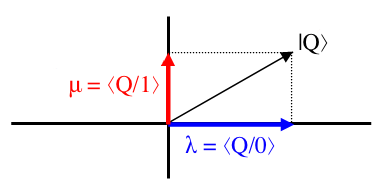
\includegraphics[scale=0.60]{images/reels}
	\end{center}
	\caption{\textit{Visualisation d'un état quantique dans le cas où $\lambda$ et $\mu$ sont des réels. introduction de la notation réduite.}}
	\label{reels}
\end{figure}

\begin{figure}
	\begin{center}
		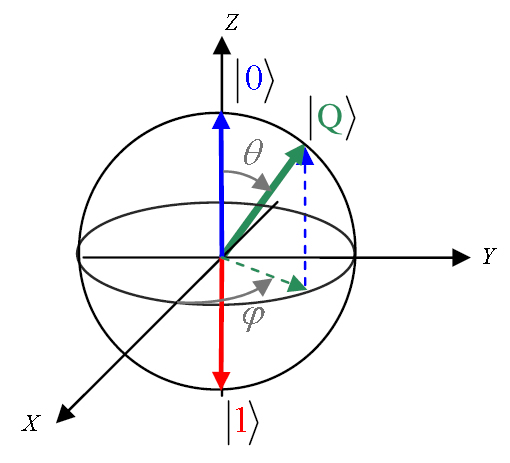
\includegraphics[scale=0.60]{images/bloch}
	\end{center}
	\caption{\textit{Visualisation d'un état quantique dans le cas où $\lambda$ et $\mu$ sont des complexes.}}
	\label{bloch}
\end{figure}

		\subsection{extension à plusieurs QuBits}

\para{
	On parle de plusieurs QuBits, mais aussi ds principes de la mécanique quantique de manière génrale (principe 1 et 2) et de l'aplitude de proba
}

	\section{Portes logiques}

%
% -----------------------
% [?] CONCLUSION
% -----------------------
%/

\chapter*{Conclusion}
\addcontentsline{toc}{chapter}{Conclusion}

\para{
	...
}

\chapter*{Bibliographie}

\para{
	...
}


\chapter*{Annexe}

\end{document}
